% \review{Request from Reviewer A:
% \begin{itemize}
% \item clarify relationship between formalization and implementation
% \item correct and address mistakes, typos, confusing terminology and code snippets
% \item address pressing questions in the paper.
% \end{itemize}}

% \review{Request from Reviewer B:
% \begin{itemize}
% \item Add details in section 5 (see above)
% \item Clarify the status of Theorem 4
% \end{itemize}}

% \review{Request from Reviewer C:
% \begin{itemize}
% \item confirmation that blame theorem issue is essentially just a typo.
% \item  clarify the policy rules wrt accessing (un)checked pointers in (un)checked regions
% \item  remove, or at least point out and justify the discrepancies between the Coq code and the paper, eg concerning Fig2
% \end{itemize}}

% \review{Request from the conditions:
% Minimal requirements for acceptance ("shepherding conditions"):
% \begin{itemize}
% \item please clarify the formalization status of Theorem 4 and the intended guarantee w.r.t. NULL 
%   dereferencing, clarify whether the code examples are intended to be actual C -- cf the discussion
%   of  pointer arithmetic and undefined behavior in review 1 -- and tweak them if necessary) 
% \item please clarify the policy of dereferencing of (un)checked pointers in (un)checked regions as pointed out by two reviewers, and address the discrepancies between the paper's calculus and the Coq formalization
% \item please include more details on the proposed model-driven random testing approach from section 5 (cf review B)
% \end{itemize}
% }

\section{Introduction}\label{sec:intros}

% \review{End of I.: a diagram would be helpful understanding how III, IV and V relate
%   to each other and to clang-checkedc}

% \review{The paper builds on the operational semantics from [21]. Even though the
%   authors explained at high-level the main extensions w.r.t. [21], it'd be great
%   to add a paragraph that discusses what are the main changes from [21] in terms
%   of the technical development (if there are any), e.g., are there any new
%   challenges that needed to be solved while proving the blame theorem for this
%   paper's semantics?}

The C programming language remains extremely popular despite the
emergence of new, modern languages. Unfortunately, C programs lack
spatial memory safety, which makes them susceptible to a host
of devastating vulnerabilities, including buffer overflows and
out-of-bounds reads/writes. Despite their long history, buffer
overflows and other spatial safety violations are among the most
prevalent and dangerous vulnerabilities on the Internet today \cite{Zeng:2013:SRF:2534766.2534798}.

% One possible solution is Checked C
% \begin{itemize}
% \item Think of it as migratory/gradual typing, but for C.
% \item Distinct pointer types, but which are backward binary- and source-compatible.
% \item Checked regions, containing only checked pointers and restricted
%   idioms, aim to ensure spatial safety
% \item Implemented as an extension to Clang/LLVM. Good performance
%   (compared to ASAN etc.)
% \end{itemize}

Several industrial and research efforts---including CCured~\cite{Necula2005},
Softbound~\cite{softbound}, and ASAN~\cite{Serebryany2012}---have
explored means to compile C programs 
to automatically enforce spatial safety. These
approaches all impose performance overheads deemed too high for
deployment use. Recently, \citet{Elliott2018} introduced \checkedc, an
open-source extension to C with new types and
annotations whose use can ensure a program’s spatial safety.
Importantly, \checkedc supports development that is 
incremental and compositional. Code regions (e.g.,
functions or whole files) designated as \emph{checked} enforce
spatial safety in a manner preserved by composition with
other checked regions. But not all regions must be checked: Checked
C's annotated \emph{checked pointers} are binary-compatible with legacy pointers, and
may coexist in the same code, which permits a deliberate (and
semi-automated) refactoring process. Parts of the FreeBSD kernel have
been successfully ported to \checkedc~\cite{duanrefactoring}, and overall, performance
overhead seems low enough for practical deployment.

While \checkedc promises to enforce spatial safety, we might wonder
whether its design and implementation deliver on this promise, or even
what ``spatial safety'' means when a program contains both checked and
unchecked code. In prior work, \citet{ruef18checkedc-incr} developed a core
formalization of \checkedc and with it proved a \emph{soundness} theorem for
checked code: any stuck (i.e., ill-defined)
state reached by a well-typed program amounts to a spatial safety
violation; such a state can always be attributed to, i.e., 
\emph{blamed on}, the execution of code that is not in a checked
region. While their work is a good start, 
it fails to model important aspects of \checkedc's functionality,
particularly those involving pointers to arrays. In this paper, we
cover this gap, making three main contributions.

\myparagraph{Dynamically bounded and null-terminated arrays}
%
Our first contribution is a core formalism called \lang, which extends
\citet{ruef18checkedc-incr} with several new features, most notably 
\emph{dynamically bounded arrays} (Section~\ref{sec:formal}). 
% First, we add important language features previously not modeled and
Dynamically bounded arrays are those whose size is
known only at run time, as designated by in-scope variables using
dependent types. A pointer's accessible memory is bounded both above
and below, to admit arbitrary pointer arithmetic.

\lang also models
\emph{null-terminated} arrays, a kind of dynamically bounded array
whose upper bound
defines the array's \emph{minimum} length---additional space is available 
up to a null terminator. For example, the \checkedc type
\lstinline{nt_array_ptr<char> p:count(n)} says that
\lstinline{p} has length \emph{at least} \lstinline{n} (excluding the
null terminator), but further capacity is present if %
\lstinline|p[n]| is not null. \checkedc (and \lang) supports flow-sensitive
\emph{bounds widening}: statements of the form \lstinline|if (*p) | $s$,
where \lstinline{p}'s type is \lstinline{nt_array_ptr<T> count(0)},
typecheck statement $s$ under the assumption that \lstinline{p} has
type \lstinline{nt_array_ptr<T> count(1)}, 
 i.e., one more than it was,
since the character at the current-known length is
non-null. Similarly, the call \lstinline|n = strlen(p)| will widen
\lstinline|p|'s bounds to \lstinline|n|. Subtyping permits treating
null-terminated arrays as normal arrays of the same size (which
does not include, and thereby protects, the null
terminator).\footnote{
    See Sec.~\ref{sec:related} for a careful comparison of
    \citet{ruef18checkedc-incr} and \lang.
}

We prove, in Coq, a blame theorem for \lang.  As far as we are aware,
ours is the first formalized type system and proof of soundness for
pointers to null-terminated arrays with expandable bounds.

% \yiyun{What about strlen? Clang doesn't do null check/bounds check on
%   strlen. We found that issue while developing our model rather than
%   through random testing. If we don't have enough bugs
%   revealed from random testing, maybe we should instead focus on the
%   under-specified or unclear behaviors from the checkedc spec that we
%   found in the process of designing the typing/semantic rules}
% \mwh{Mentioned strlen above. How should we change what's written?}

\myparagraph{Sound compilation of checked pointers} Our second
contribution is a formalization of bounds-check insertion for array
accesses (Section~\ref{sec:compilation}). Our operational semantics
annotates each pointer with metadata that describes its bounds, and
the assignment and dereference rules have premises to confirm the
access is in bounds. An obvious compilation scheme (taken by
Cyclone~\cite{Jim2002,GrossmanMJHWC02}, CCured~\cite{Necula2005}, and
earlier works) would be to translate annotated pointers to multi-word
objects: one word for the pointer, and 1-2 words to describe its lower
and upper bounds. Inserted checks reference these bounds. While
convenient, such ``fat'' pointers are expensive, and break backward
binary compatibility with legacy pointers.

  To show that pointer annotations can be safely
  erased, and thus fat pointers are not needed, we formalize a
  translation of \lang to \elang, which is an 
  untyped version of \lang that drops metadata annotations, and
  lacks bounds/null checks in the semantics rules. Instead,
  the compilation process inserts null/bounds checks explicitly, leveraging
  compile-time type information. While we do not definitively prove
  it, we provide strong evidence that compilation is correct. We use PLT
  Redex~\cite{pltredex} to mechanize (a generalization of) \lang, 
  \elang, and compilation between the two, and we use randomized testing 
to validate that the compiled program \emph{simulates} the
original. In addition to demonstrating the technical point that metadata
annotations in the \lang formalism do not necessitate fat pointers,
compilation also sheds light on the actual Checked C compilation
process. 
% \review{ Beginning of page 2: "we show", then "give confidence". I am left confused as
%   to whether the CoreChkC --> CoreC compilation is shown correct (theorem with
%   proof), or carefully debugged and tested in plt-redex (which is fine too, I
%   just find the choice of terminology confusing)}
% \liyi{typo, should be "validate through randomized testing"}

As far as we are aware, \lang is the first formalism to cleanly
separate bounds-checking compilation from the core semantics; prior
work~\cite{Feng2006,Condit2007} merged the two, conflating
\emph{meaning} with \emph{mechanism}. In carrying out the
formalization, we discovered that our compilation approach for
null-terminated array pointers is more expressive than that proposed
in the Checked C specification~\cite{checkedc}
(Section~\ref{sec:disc}); we would not have discovered this
improvement had we not separated checks from semantics.
%\leo{Either checks from semantics or the checks from the semantics.
%  Not sure what I prefer phrasing wise...}

% The second contribution is a presentation of the semantics of
% dynamically bounded arrays that simplifies formal reasoning. 
% \mwh{I don't follow what's here. Want to change this to be about the
%   clean separation of semantics metadata from obligating the compiler
%   to include it as fat pointers.}
% We design our type system to closely model the behavior of the
% \checkedc specification. However, we choose to diverge slightly from the
% \checkedc semantics by utilizing stack variables to keep additional
% bounds information that cannot be expressed with a simple type
% system that does not support theorem proving. Due to
% the limitation that \checkedc functions must be binary compatible with
% C, we cannot explicitly pass bounds to functions. We make a
% comprimise and restrict the more accurate bounds information to be
% accessible only within the stack frame where the checked array pointer
% is defined. As we will see, despite this restriction, the user can
% write significantly more expressive code that would not be
% possible with the existing \checkedc specification.
% As far as we know, prior systems \yiyun{what
%   systems? the current checkedc spec is clearly one of them. What
%   about Deputy?} 
% \yiyun{widening of null-terminated array pointers at the current
%   stacck frame}
% take a more conservative approach and insert checks completely based
% on bounds determined at compile time. 
%  
% \mwh{merge the following and the above into one para/contribution}
% By introducing this new mechanism of bounds tracking through stack
% variables, we run the risk of accidentally using ``fat pointers'' in
% our formalism, where every the heap and literals are annotated with
% types. To ensure our system does not access bounds information that is
% not supposed to be accessible at runtime, we compile from \lang into
% \elang, where the expressions are free of bounds annotations and the
% dynamic checks and widening expressions are made explicit. We prove
% the blame theory using the annotated language \lang, and then prove
% that \lang are \elang are bisimilar. \yiyun{Maybe discuss its
%   impact on proof engineering? We don't have the full proofs yet so not
%   sure how to comment on that.}

% define the semantics of the source language via compilation to a
% target where the checks are made manifest. We'd prefer the semantics
% are made directly manifest as operational rules, and we followed this
% approach, taken by the earlier formal work. However, we found that the
% addition of dynamic sizes complicates this approach---seems to require
% ``fat pointers.'' So: We developed a compiler to a system without
% bounds annotations and proved it bisimilar to the one with
% annotations.

\myparagraph{Model-based randomized testing} Our third and final
contribution is a strategy and implementation of model-based
randomized testing (Section~\ref{sec:evaluation}).  To check the
correctness of our formal model, we compare the behavior between the
existing Clang \checkedc implementation and our own model. This is
done by a conversion tool that converts expressions from \lang into
actual \checkedc code that can be compiled by the Clang \checkedc
compiler. We build a random generator of programs largely based on the
typing rules of \lang and make sure that, both statically and
dynamically, \lang and Clang Checked C are consistent after
conversion.  This helped rapidly prototype the model and uncovered
several issues in the Checked C compiler.

\begin{figure}
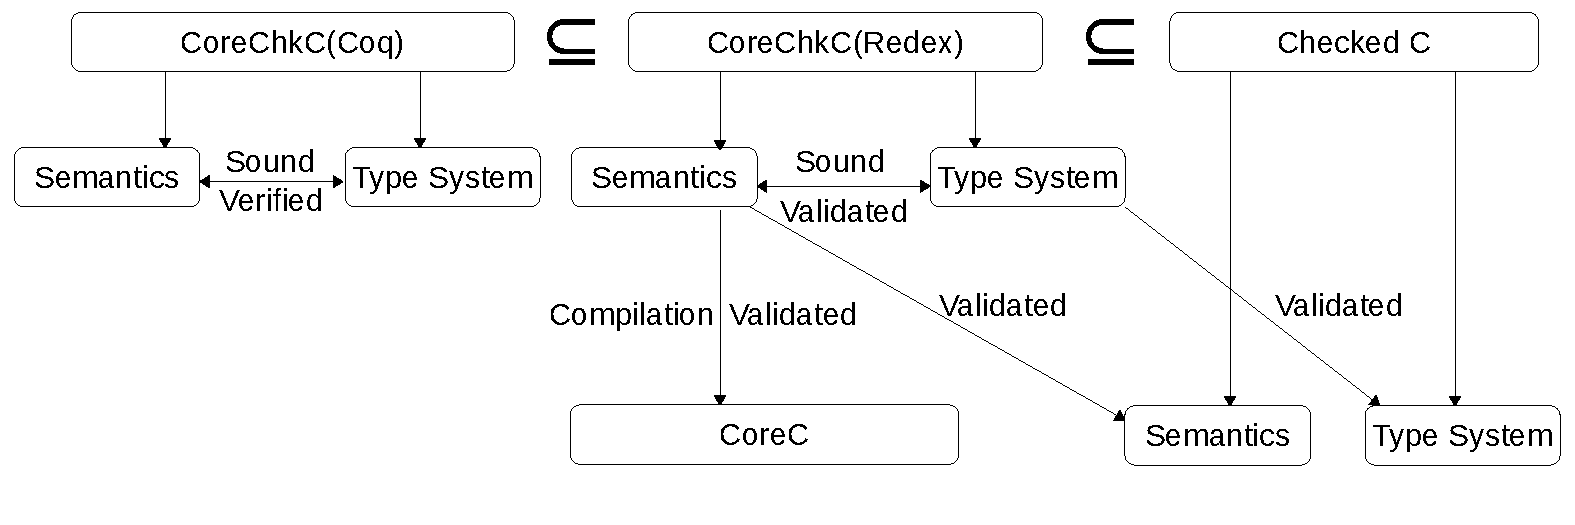
\includegraphics[width=0.5\textwidth]{relationship.pdf}
\caption{
    \lang models' relationship to \checkedc
}
  \label{fig:model-relation}
\end{figure}

  \myparagraph{Summary Visualization} The
  relationship among our contributions is visualized in
  Fig.~\ref{fig:model-relation}. With the Coq model of \lang we prove
  soundness (and with it, \emph{blame}) of the \checkedc type system
  and semantics. With the Redex model, we use randomized testing to
  validate both type soundness and compilation correctness, where the
  latter shows how compilation need not output fat pointers despite
  the use of pointer annotations in the \lang model. The Redex \lang
  model is also the basis of randomized testing of the correctness of
  the \checkedc compiler implementation, both its type checker and the
  semantics of its emitted code, at least for the subset of the
  language in the Redex model. The Redex model's syntax
  is slightly richer than the Coq version: conditional guards and
  function arguments may be arbitrary expressions, where the Coq
  version limits them to constants and variables, making handling of
  dependent types a bit simpler. We find a useful synergy between the
  Coq and Redex models for carrying out a language development. The
  richer, executable Redex model is useful for quickly modeling and
  testing new features, both formally and against a real
  implementation. Once solidified, new features can be added to the
  Coq model (perhaps somewhat simplified) for final proofs of
  correctness.

We begin with a review of \checkedc (Section~\ref{sec:overview}),
present our main contributions
(Sections~\ref{sec:formal}--\ref{sec:evaluation}), and conclude with a
discussion of 
related and future work (Sections~\ref{sec:related},
\ref{sec:conclude}). All code and proof artifacts (both for Coq and
Redex) can be found at \url{https://github.com/plum-umd/checkedc}. 


% In this paper, we develop a NULL-terminated (NT) checked pointer type
% in Checked C, whose syntax is \lstinline{nt_array_ptr<T>} (for any type
% \lstinline{T}) \yiyun{we didn't model anything besides a single
%   numeric type but what's the meaning of an ntarray when T /=
%   char? If it was int, then it implicitly rules out the possibility of
% storing 0}. Programmers familiar with C's standard string library will
% be quite familiar with NT pointers. But spatially safe NT pointers are
% not present in modern type-safe languages (such as Java, Scala,
% Haskell, Rust, etc.), which typically pair dynamically-sized buffers
% with metadata to indicate the buffer's length and capacity. While some
% prior safe-C implementations (such as CCured, Cyclone, and Deputy)
% have supported NT pointers, no prior work of which we are aware has
% formalized and proved them safe, nor has it assessed \yiyun{did we
%   assess anything?} their performance
% against non-NT alternatives. We fill these gaps in this work.

% In this paper we formalize Checked C with checked NT pointers and
% re-prove our compositional proof of blame (done in the Coq proof
% assistant); our formalism also includes lightweight dependent and
% function types, and other extensions. We have also implemented checked
% NT pointers in the Checked C compiler, and evaluated their
% effectiveness on a series of benchmarks; we use these benchmarks to
% show the advantages of our support compared to refactoring the code to
% use normal arrays. \yiyun{I don't think we ever evaluated nt-array
%   pointer against ordinary array pointers. It's more of a legacy code
%   issue since C uses nt-array in its stdlib} Our implementation, code, and benchmarks are (or
% will be) available in the Checked C Github repository.


% Intro:
% \begin{itemize}
% \item NULL-terminated arrays are a feature long-present in
%   C. Low-overhead way of implementing expandable buffers.
% \item But: Spatially-safe languages have typically eschewed such
%   arrays in favor of traditional, bounds-checked arrays. For example,
%   Java Strings are not zero-terminated (I think)
% \item Some considerations in past languages, like Cyclone, CCured, and
%   Deputy, but never formalized and proved correct.
% \item Checked C is backward compatible with C, so we need to
%   incorporate NT arrays.
% \end{itemize}
